%15 min preso!
\documentclass[xcolor=table,aspectratio=169]{beamer}
\usepackage{beamerthemesplit}
\usepackage{wrapfig}
\usetheme{SPbGU}
\usepackage{pdfpages}
\usepackage{amsmath}
\usepackage{cmap}
\usepackage[T2A]{fontenc}
\usepackage[utf8]{inputenc}
\usepackage[english]{babel}
\usepackage{indentfirst}
\usepackage{amsmath}
\usepackage{tikz}
\usepackage{multirow}
\usepackage[noend]{algpseudocode}
\usepackage{algorithm}
\usepackage{algorithmicx}
\usepackage{fancyvrb}
\usepackage{hyperref} 
\usetikzlibrary{calc}
\usetikzlibrary{shapes, backgrounds}
\usetikzlibrary{arrows,automata}
\usetikzlibrary{positioning}
\usetikzlibrary{fit}
\usetikzlibrary{shapes.callouts}
\usetikzlibrary{shapes.misc}
\usepackage{xparse}
\usepackage{fontawesome}

\usepackage{etoolbox,refcount}
\usepackage{multicol}

\usepackage{tabularx}
\newcolumntype{Y}{>{\raggedleft\arraybackslash}X}

\renewcommand{\thealgorithm}{}

\newtheorem{mytheorem}{Theorem}
\renewcommand{\thealgorithm}{}

\newcommand{\tikzmark}[1]{\tikz[overlay,remember picture] \node (#1) {};}
\def\Put(#1,#2)#3{\leavevmode\makebox(0,0){\put(#1,#2){#3}}}

\newcommand{\ltz}{$< 1$}

\tikzset{
    state/.style={
           rectangle,
           rounded corners,
           draw=black, very thick,
           minimum height=2em,
           inner sep=2pt,
           text centered,
           },
}

\tikzset{
    invisible/.style={opacity=0,text opacity=0},
    visible on/.style={alt=#1{}{invisible}},
    alt/.code args={<#1>#2#3}{%
      \alt<#1>{\pgfkeysalso{#2}}{\pgfkeysalso{#3}} % \pgfkeysalso doesn't change the path
    },
}

\tikzset{cross/.style={cross out, draw=black, minimum size=2*(#1-\pgflinewidth), inner sep=0pt, outer sep=0pt, ultra thick},
%default radius will be 1pt. 
cross/.default={1pt}}

\NewDocumentCommand{\mycallout}{r<> O{opacity=0.8,text opacity=1} m m m}{%
\tikz[remember picture, overlay]\node[align=center, fill=cyan!20, text width=#5cm,
#2,visible on=<#1>, rounded corners,
draw,rectangle callout,anchor=pointer,callout relative pointer={(290:0.5cm)}]
at (#3) {#4};
}

\NewDocumentCommand{\mycalloutR}{r<> O{opacity=0.8,text opacity=1} m m m}{%
\tikz[remember picture, overlay]\node[align=center, fill=cyan!20, text width=#5cm,
#2,visible on=<#1>, rounded corners,
draw,rectangle callout,anchor=pointer,callout relative pointer={(30:0.8cm)}]
at (#3) {#4};
}


%callout relative pointer={(230:0.5cm)}]

\newcounter{countitems}
\newcounter{nextitemizecount}
\newcommand{\setupcountitems}{%
  \stepcounter{nextitemizecount}%
  \setcounter{countitems}{0}%
  \preto\item{\stepcounter{countitems}}%
}
\makeatletter
\newcommand{\computecountitems}{%
  \edef\@currentlabel{\number\c@countitems}%
  \label{countitems@\number\numexpr\value{nextitemizecount}-1\relax}%
}
\newcommand{\nextitemizecount}{%
  \getrefnumber{countitems@\number\c@nextitemizecount}%
}
\newcommand{\previtemizecount}{%
  \getrefnumber{countitems@\number\numexpr\value{nextitemizecount}-1\relax}%
}
\makeatother    
\newenvironment{AutoMultiColItemize}{%
\ifnumcomp{\nextitemizecount}{>}{3}{\begin{multicols}{2}}{}%
\setupcountitems\begin{itemize}}%
{\end{itemize}%
\unskip\computecountitems\ifnumcomp{\previtemizecount}{>}{3}{\end{multicols}}{}}


\beamertemplatenavigationsymbolsempty

\title[FLDDA Research Group Report]{Formal Language Driven Data Analysis Research Group Report}
\institute[SPbSU]{
Saint Petersburg State University
}

% То, что в квадратных скобках, отображается в левом нижнем углу.
\author[Semyon Grigorev]{Semyon Grigorev}

\date{February 29, 2024}


%Я предлагаю сначала в общем рассказать интересы и компетенции группы, 
%что научная группа сделала за 3 месяца, 
%потом потратить 1 страницу презентации на каждого из студентов (что сделал, почему важно для Yiming, какие планы). 
%В конце перейти к планам на год.

\begin{document}
{
\begin{frame}[fragile]
  \begin{table}
  \centering
  %
\includegraphics[height=1.5cm]{pictures/SPbGU_Logo.png}
  \begin{tabularx}{\linewidth}{XcX}
    
\includegraphics[height=0.9cm]{pictures/hu_logo.jpeg} \hfill
    & 
    & \hfill 
\includegraphics[height=1.6cm]{pictures/SPbGU_Logo.png}
  \end{tabularx}
  \end{table}
  \titlepage
\end{frame}
}

\begin{frame}[fragile]
  \frametitle{Research Landscape}  
  \begin{itemize}
    \item AI-guided symbolic execution
    \begin{itemize}
      \item Ekaterina Shemetova
      \item Maxim Nigmatulin
      \item Anna Chistiakova
      \item Semyon Grigorev
      \item Collaboration with Dmitriy Mordvinov and Vadim Lomshkov
    \end{itemize} 
    \item Parsing Techniques
    \begin{itemize}
      \item Ivan Lomikovskiy
      \item Semyon Grigorev
      \item Collaboration with Kirill Prazdnikov and Pavel Pertsev
    \end{itemize}
  \end{itemize} 
  
\end{frame}


\begin{frame}[fragile]
  \frametitle{$\mathcal{AI}$-Guided Symbolic Execution}  
  \begin{itemize}
    \item[\faCheck] Reusable infrastructure for training developed and implemented
      \begin{itemize}
        \item Wrapper for SVM to convert it to server
        \item Python client --- $\mathcal{AI}$ agent to training
        \item Basic manipulation with neural networks 
      \end{itemize}
    \item[\faCheck] Basic dataset for train and validation/test
    \item[\faCheck] Basic performance tuning
    \item[\faCheck] First version of $\mathcal{AI}$ agent which guide SVM
    \begin{itemize}
      \item Can be used in various engines: we use language-independent features 
    \end{itemize}
    \item[\faGears] Dataset extension
    \item[\faGears] GNN quality improvement 
  \end{itemize}
\end{frame}

\begin{frame}[fragile]
  \frametitle{$\mathcal{AI}$-Guided Symbolic Execution: Preliminary results}  
  \begin{itemize}
    \item 190 methods: algorithms, data structures, real-world projects
    \item AI --- our AI-based agent
    \item ETCC (ExecutionTreeContributedCoverage) --- one of the best algorithmic strategies
  \end{itemize}
  \onslide<2->{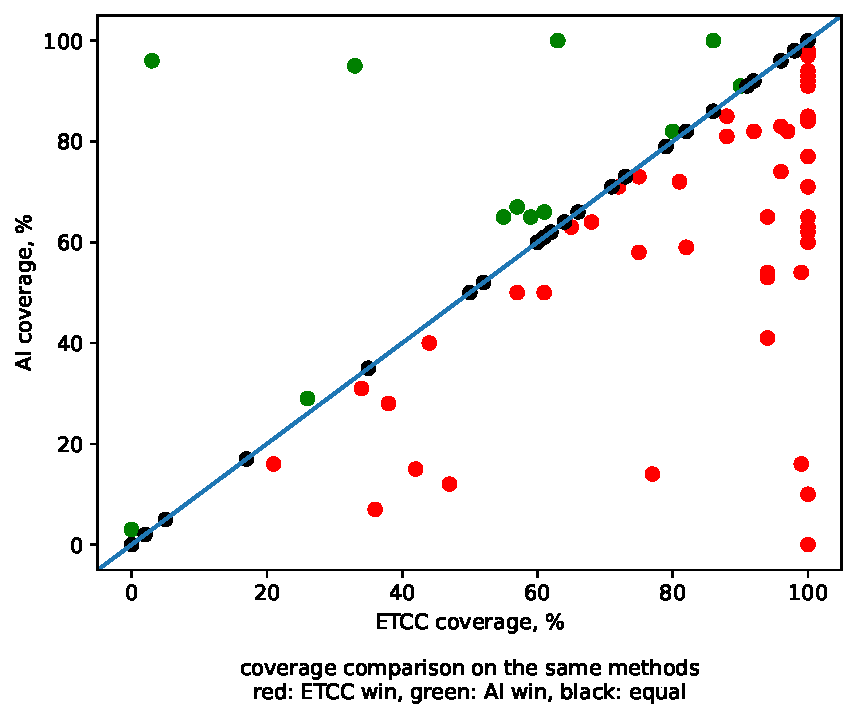
\includegraphics[width=0.3\textwidth]{pictures/coverage.pdf}}
  \onslide<3->{
    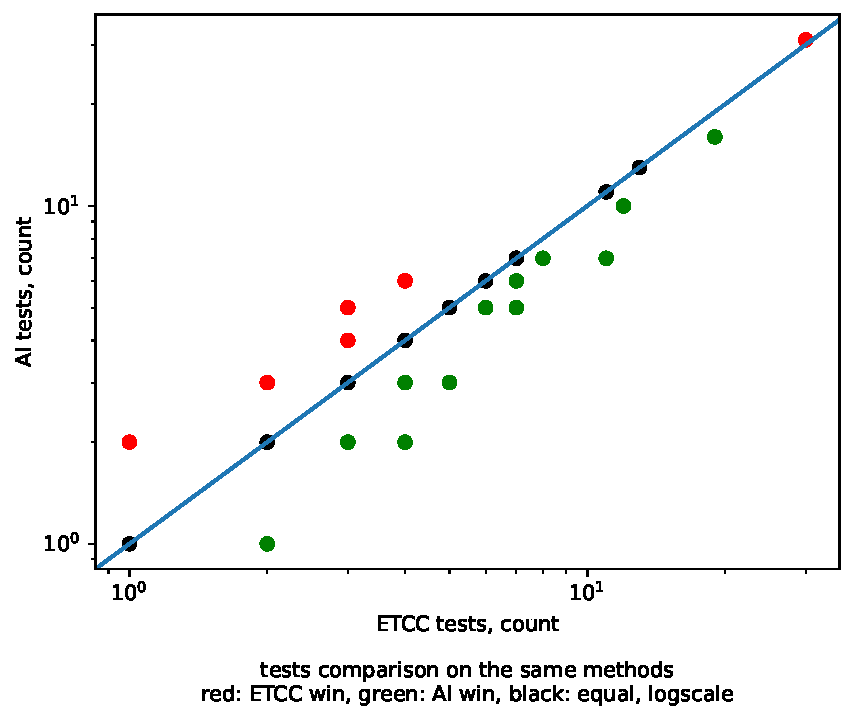
\includegraphics[width=0.3\textwidth]{pictures/tests_eq_coverage.pdf}
    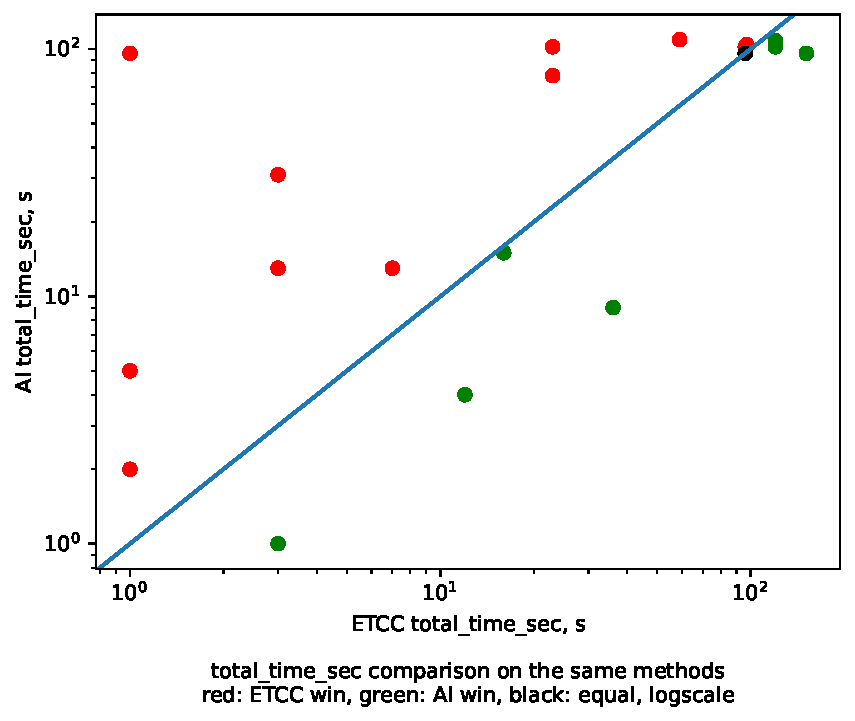
\includegraphics[width=0.3\textwidth]{pictures/total_time_eq_coverage.pdf}
  }
  \begin{itemize}
    \onslide<2->{\item Same coverage: 132, AI less: 46, AI more: 12}
    \onslide<3->{\item For same coverage: less tests, comparable time}
  \end{itemize}
\end{frame}


\begin{frame}[fragile]
  \frametitle{Parsing Techniques}  
  \begin{itemize}
    \item[\faCheck] Basic parser development tool is created
    \begin{itemize}
      \item[\faCheck] Preliminary performance evaluation 
    \end{itemize}
    \item[\faCheck] Error recovery mechanism
    \begin{itemize}
      \item[\faGears] Preliminary performance evaluation 
    \end{itemize} 
    \item[\faHourglassHalf] Advanced incremental parsing
    \item[\faHourglassHalf] Advanced scannerless mode
  \end{itemize}
\end{frame}

\begin{frame}[fragile]
  \frametitle{Parsing Techniques: Preliminary Evaluation Result}  
  \begin{itemize}
    \item Java grammar
    \item 3 real-world projects
    \begin{itemize}
      \item junit4: 425 files, avg. size 3KB (40KB max)
      \item guava:  1 416 files, avg size 8KB (198KB max)
      \item elasticSearch: 14 685 files, avg size 6KB (242KB max)
    \end{itemize}
  \end{itemize}
  \begin{center}
    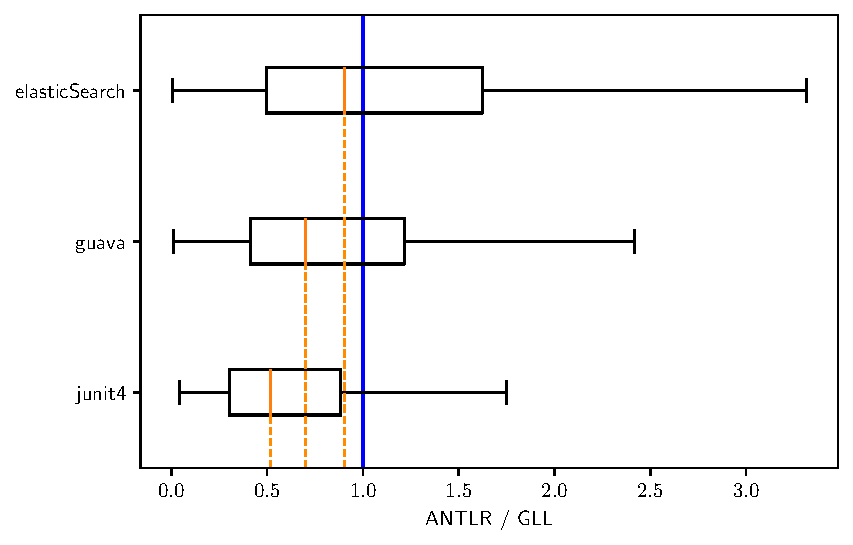
\includegraphics[width=0.5\textwidth]{pictures/gll_results.pdf}
  \end{center}
  
\end{frame}



\end{document}
